\section{Physical Optical Layer}\label{sec:optics}
\subsection{Link Budget, Receiver and Coding}
The received power of endpoint $a$ is
\begin{equation}
P_a=P_{0,a}\,G_a\,\exp\!\Big(-\frac{2\|x_a+b_a+\xi_a\|^2}{\alpha^2}\Big),
\end{equation}
with residual pointing $x_a$, hidden bias $b_a$, tracking jitter $\xi_a\sim\mathcal N(0,\sigma_\xi^2 I)$, attenuation $G_a$, and $1/e^2$ half-angle $\alpha=\mathrm{FWHM}/\sqrt{2\ln2}$. The nominal power $P_{0}$ follows from
\begin{equation}
P_0=\underbrace{P_t L_t}_{\text{Tx}}\ \underbrace{\tfrac{16\ln2}{\mathrm{FWHM}^2}}_{G_t}\ \underbrace{\tfrac{1}{4\pi r^2}}_{\text{range}}\ \underbrace{A_rL_r}_{\text{Rx}},
\end{equation}
which for $P_t=5$~mW, $L_t=-1$~dB, FWHM $=380\urad$, a 10~mm aperture, $L_r=-5.2$~dB and $r=1$~km gives $P_0=0.576\,\mu$W and $\alpha=322.7\urad$ (Table~\ref{tab:optics}). The receiver is a PIN photodiode with a transimpedance front end (thermal, shot and background noise) and on-off keying, giving the bit-error rate $\mathrm{BER}=\tfrac12\mathrm{erfc}(Q/\sqrt2)$ with $Q=I_1/(\sigma_0+\sigma_1)$. A shortened Reed--Solomon code RS(88,72) over GF$(2^8)$ corrects $t=8$ symbols~\cite{reed1960}, so a codeword (packet) is lost with probability $\sum_{k>t}\binom{n}{k}p_s^k(1-p_s)^{n-k}$, where $p_s=1-(1-\mathrm{BER})^8$. The link-availability threshold is not an input: it is the power where the packet error equals 0.1, $0.112\,\mu$W ($-39.5$~dBm), leaving a nominal margin of 7.1~dB. Fig.~\ref{fig:receiver} shows both error curves.

\begin{figure}[!t]
\centering
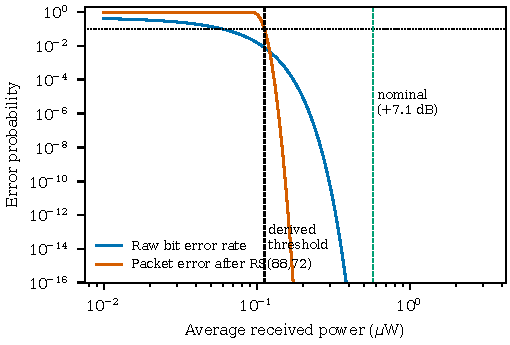
\includegraphics[width=\columnwidth]{figures/fig_v2_receiver.pdf}
\caption{Receiver model: raw bit-error rate and packet error after RS(88,72) versus average received power. The dashed lines mark the derived availability threshold and the nominal operating power.}
\label{fig:receiver}
\end{figure}

\subsection{Lock, Acquisition and Terminal Dynamics}
Each terminal tracks only while power stays above the threshold. A lock is lost after 0.5~s below it. Re-acquisition requires power at least 1.5 times the threshold for an acquisition dwell (3~s nominal, 15~s in a stress case), and a link carries packets only when both terminals are locked. The terminal is two cascaded 0.03~s lags with a 0.035~rad/s rate limit, tracking jitter $\sigma_\xi=10\urad$ RMS (35~$\mu$rad in a stress case), and encoder noise of $5\urad$. A local pilot dither and a Gaussian power fit estimate boresight bias; the fit-acceptance residual (0.20) was set on development seeds.

\begin{table}[!t]
\caption{Optical-layer parameters and their provenance}
\label{tab:optics}
\centering\footnotesize
\begin{tabular}{@{}p{0.40\columnwidth}p{0.52\columnwidth}@{}}
\toprule
Parameter & Value (source)\\
\midrule
Beam FWHM & $380\urad$ (NASA TBIRD, on-orbit measurement~\cite{schieler2023})\\
Body pointing jitter & $<10\urad$ RMS nominal~\cite{schieler2023icsos}; $35\urad$ stress (20--35~$\mu$rad uplink tracking~\cite{schieler2023})\\
Pull-in time & 3~s nominal (assumed); 15~s stress (TBIRD 10--30~s~\cite{schieler2023})\\
Tx power / losses & 5~mW; $-1$~dB Tx, $-5.2$~dB Rx (design, assumed)\\
Receiver, code & responsivity 0.9~A/W, 5~pA/$\sqrt{\text{Hz}}$, 100~Mbps OOK; RS(88,72) (design)\\
Lock hysteresis & 0.5~s loss hold, $1.5\times$ re-acquire (assumed)\\
Derived threshold & 0.112~$\mu$W at packet error 0.1\\
\bottomrule
\end{tabular}
\end{table}

\subsection{Validation Against Published NASA Data}
Table~\ref{tab:tbird} reproduces the downlink irradiance budget published for TBIRD at $30^\circ$ elevation~\cite{schieler2023} with the same budget function the crosslink simulator calls. The model total of $-52.97$~dB\,W/m$^2$ differs from the published $-52.9$ by 0.07~dB, and no line item differs by more than 0.15~dB.

\begin{table}[!t]
\caption{TBIRD downlink irradiance budget: published~\cite{schieler2023} versus the simulator's budget code}
\label{tab:tbird}
\centering\footnotesize
\begin{tabular}{@{}lrrr@{}}
\toprule
Item & Published & Model & Diff.\\
\midrule
Tx optical power, 0.9~W (dBW) & $-0.5$ & $-0.46$ & 0.04\\
Tx optics loss (dB) & $-0.3$ & $-0.30$ & 0.00\\
Tx gain, 380~$\mu$rad (dBi) & 79.0 & 78.85 & $-0.15$\\
Pointing loss, 50~$\mu$rad (dB) & $-0.2$ & $-0.21$ & $-0.01$\\
Range loss, 930~km (dB/m$^2$) & $-130.4$ & $-130.36$ & 0.04\\
Atmospheric loss (dB) & $-0.5$ & $-0.50$ & 0.00\\
\midrule
Irradiance (dB\,W/m$^2$) & $-52.9$ & $-52.97$ & $-0.07$\\
\bottomrule
\end{tabular}
\end{table}

\emph{What is real and what is modelled.} The budget, beam width, jitter range, pull-in range and the existence of a hard FEC threshold (about $-38$~dBm in the 200~Gbps mode) are published NASA/MIT-LL values. The 1~km crosslink geometry, the 100~Mbps receiver, the RS code, the lock thresholds and the transmitter power are modelled. Raw flight telemetry from NASA is not public, and we found no public ISRO inter-satellite-link data, so none is used. The validation therefore tests the link-budget arithmetic and calibrates the model; it is not a validation of the whole closed loop against flight data.

